\documentclass{homework}
\usepackage[utf8]{inputenc}
\usepackage{xspace,color,url,listings,graphicx,float,amsmath,amssymb,braket,subcaption}
\graphicspath{{./graphs/}} %location of images

\lstset{commentstyle=\color{red},keywordstyle=\color{black},
showstringspaces=false}
\lstnewenvironment{rc}[1][]{\lstset{language=R}}{}
\newcommand{\ri}[1]{\lstinline{#1}}  %% Short for 'R inline'

\lstset{language=R}             % Set R to default language

\newcommand{\hwname}{Shara Duong, Charles Colgan, Josh Borders}
\newcommand{\hwnum}{1}

\newcommand{\hwtype}{Homework}
\newcommand{\hwclass}{MATH 6350}

\begin{document}

\maketitle

Contributions

Charles Colgan created figures 2 through 5, wrote and edited code for all questions, wrote and edited text for all questions.
Josh Borders created figure 1, created the tables containing R output, and wrote and edited text for all questions.
Shara Duong wrote and edited code for all questions, wrote and edited text for some questions.

%Question 1
\question
The following table displays the respective means and standard deviations of each feature in the Auto data set These are the number of Cylinders, Displacement (in\textsuperscript{3}), Horsepower, Weight (lbs), and Acceleration (seconds required to accelerate from 0mph to 60mph). The total number of case studies was 392.
\begin{rc}
           Cyl   Displ        HP    Weight     Accel
Mean   5.471939 194.412 104.46939 2977.5842 15.541327
StdDev 1.705783 104.644  38.49116  849.4026  2.758864
\end{rc}

%Question 2
\question
\begin{figure}[H]
\centering
\subfloat[]{\includegraphics[width=5cm,height=4cm]{graphs/histmpg.pdf}}
\subfloat[]{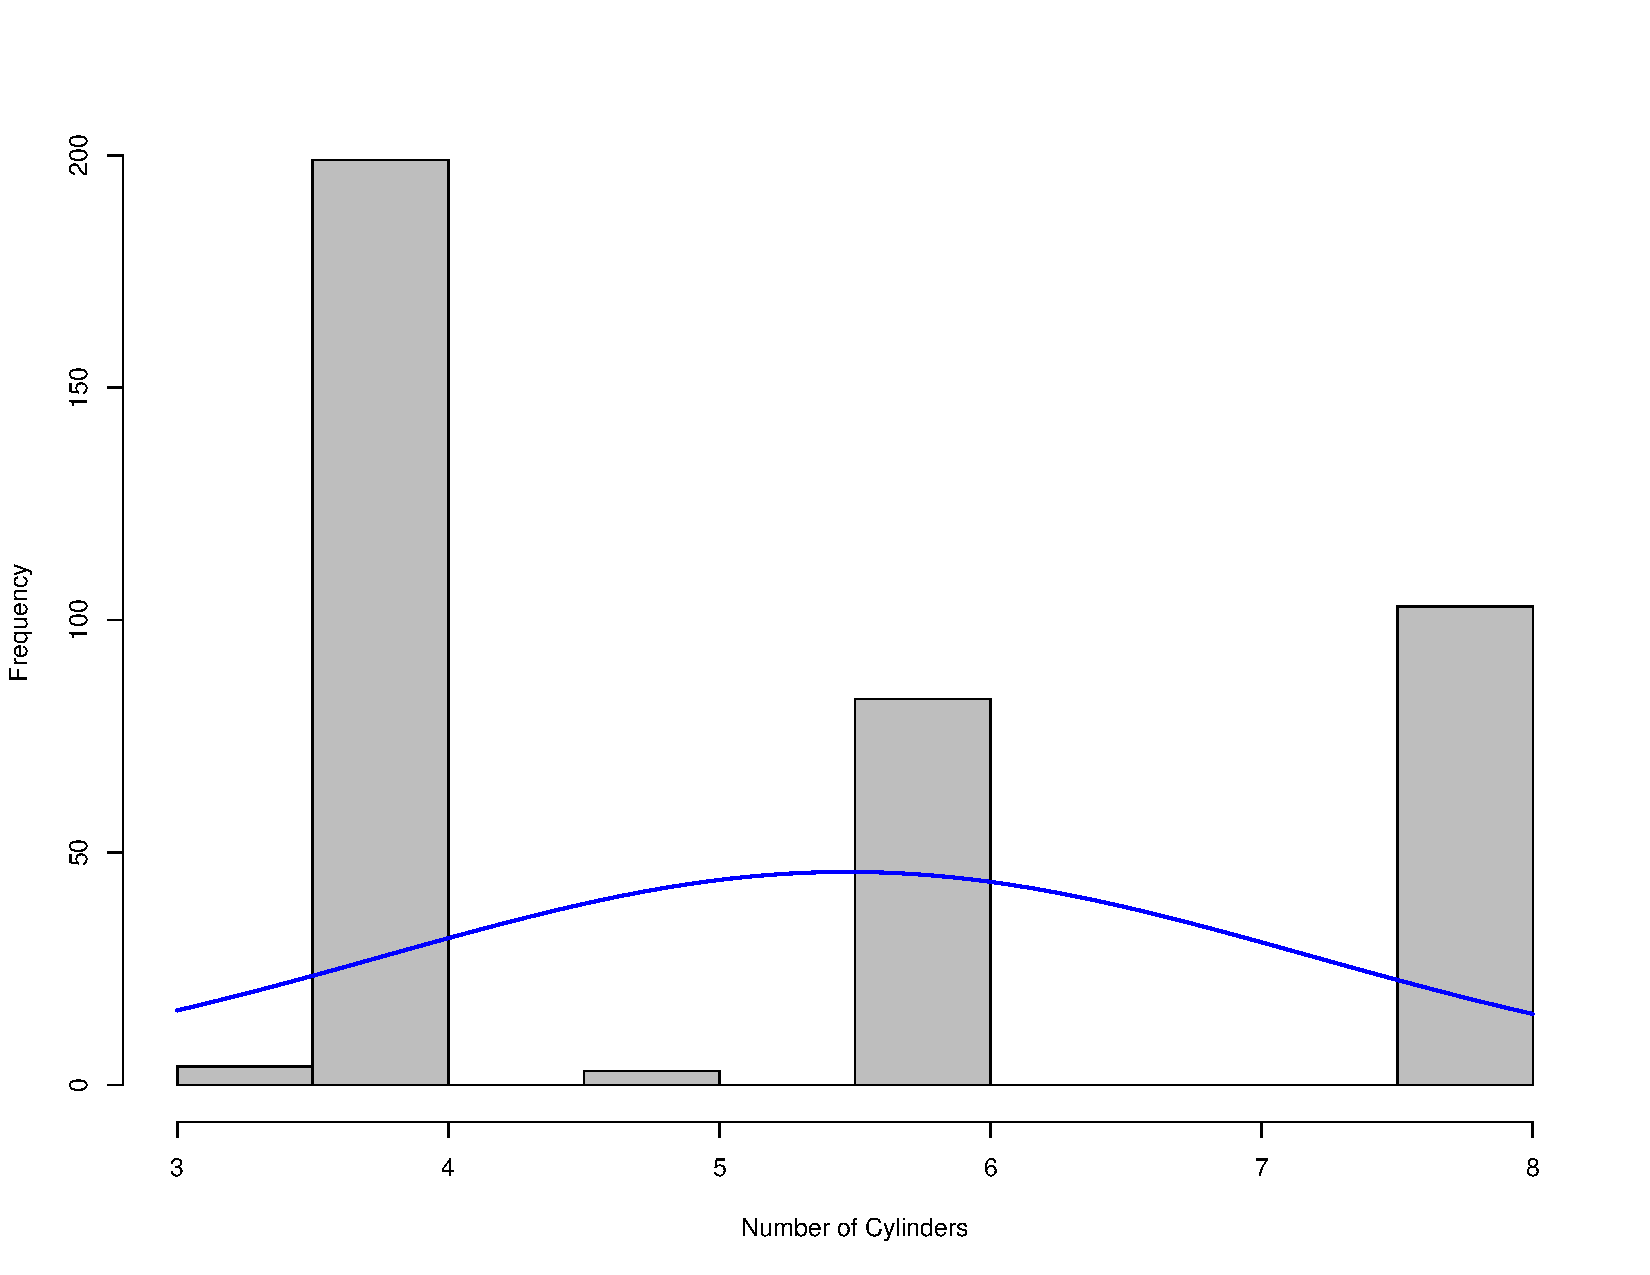
\includegraphics[width=5cm,height=4cm]{graphs/histCyl.pdf}}
\subfloat[]{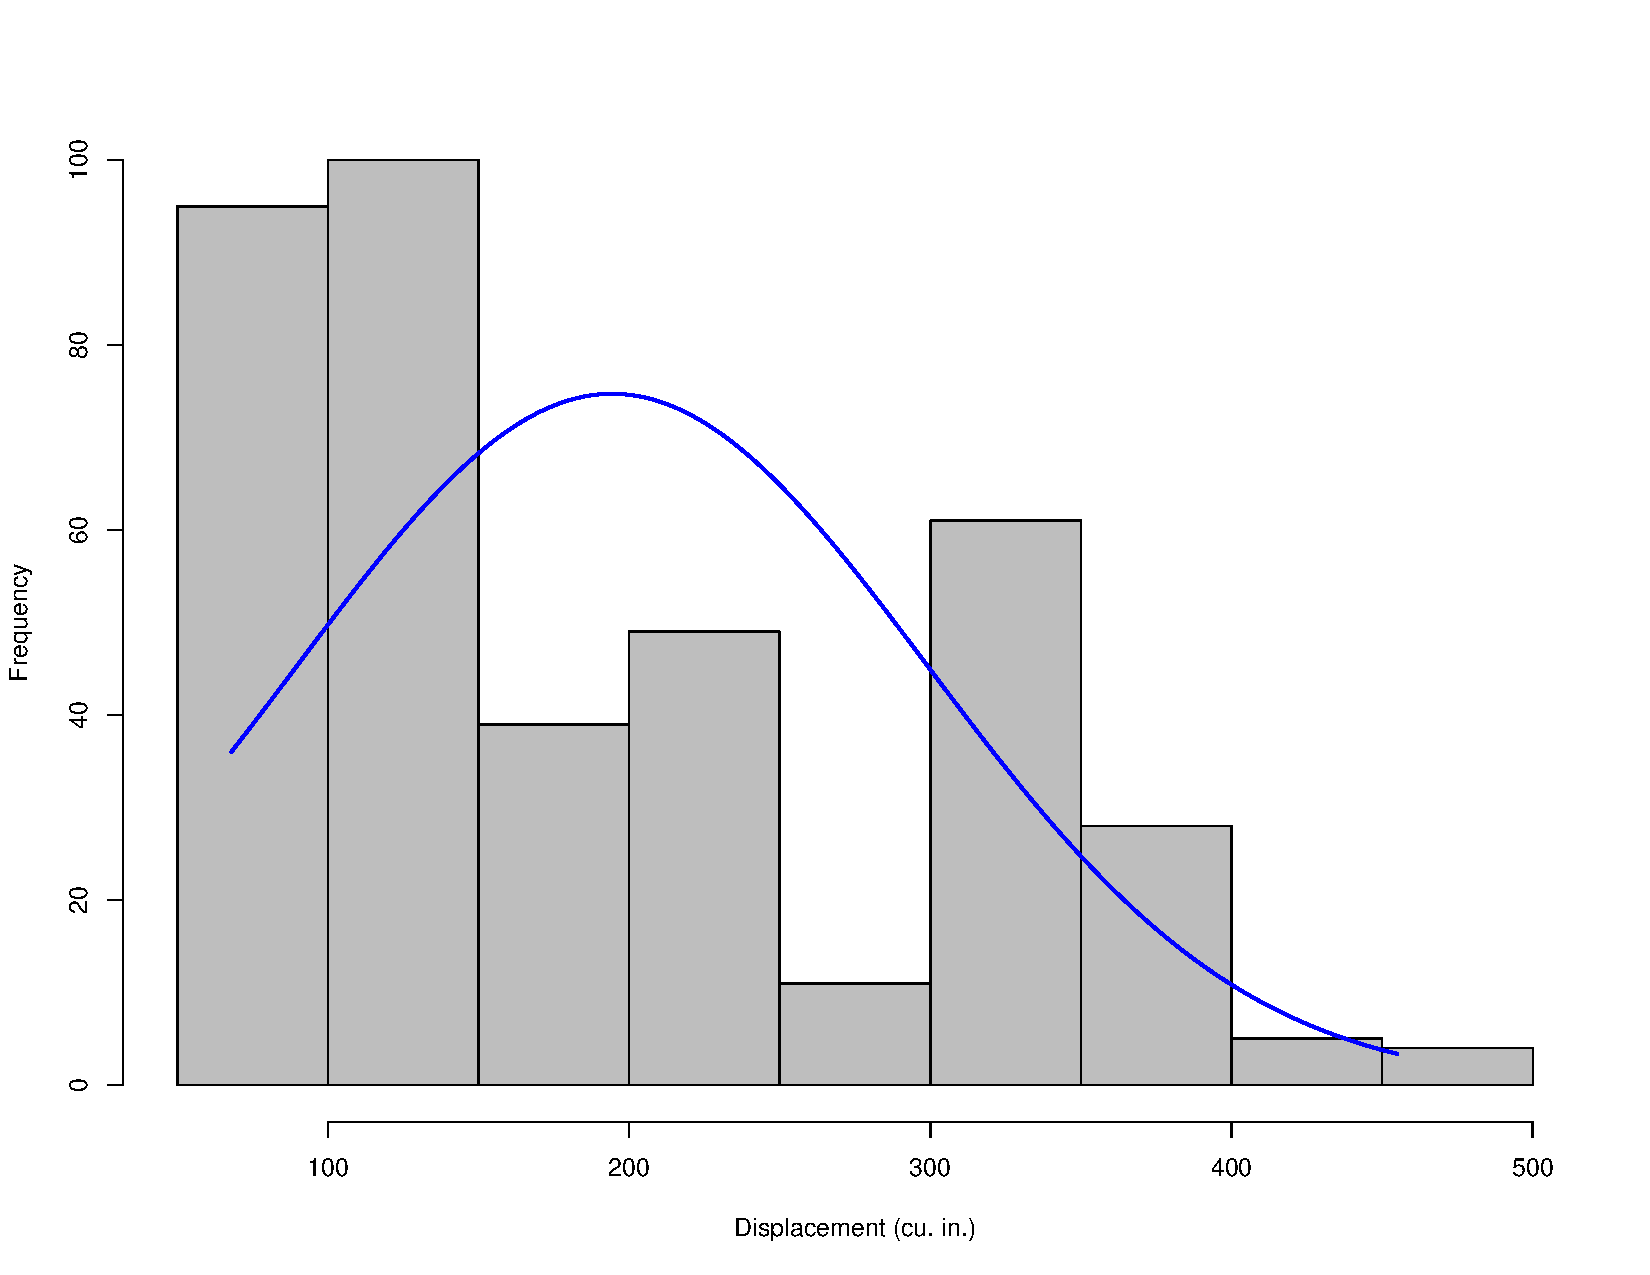
\includegraphics[width=5cm,height=4cm]{graphs/histDis.pdf}}\\
\subfloat[]{\includegraphics[width=5cm,height=4cm]{graphs/histHp.pdf}}
\subfloat[]{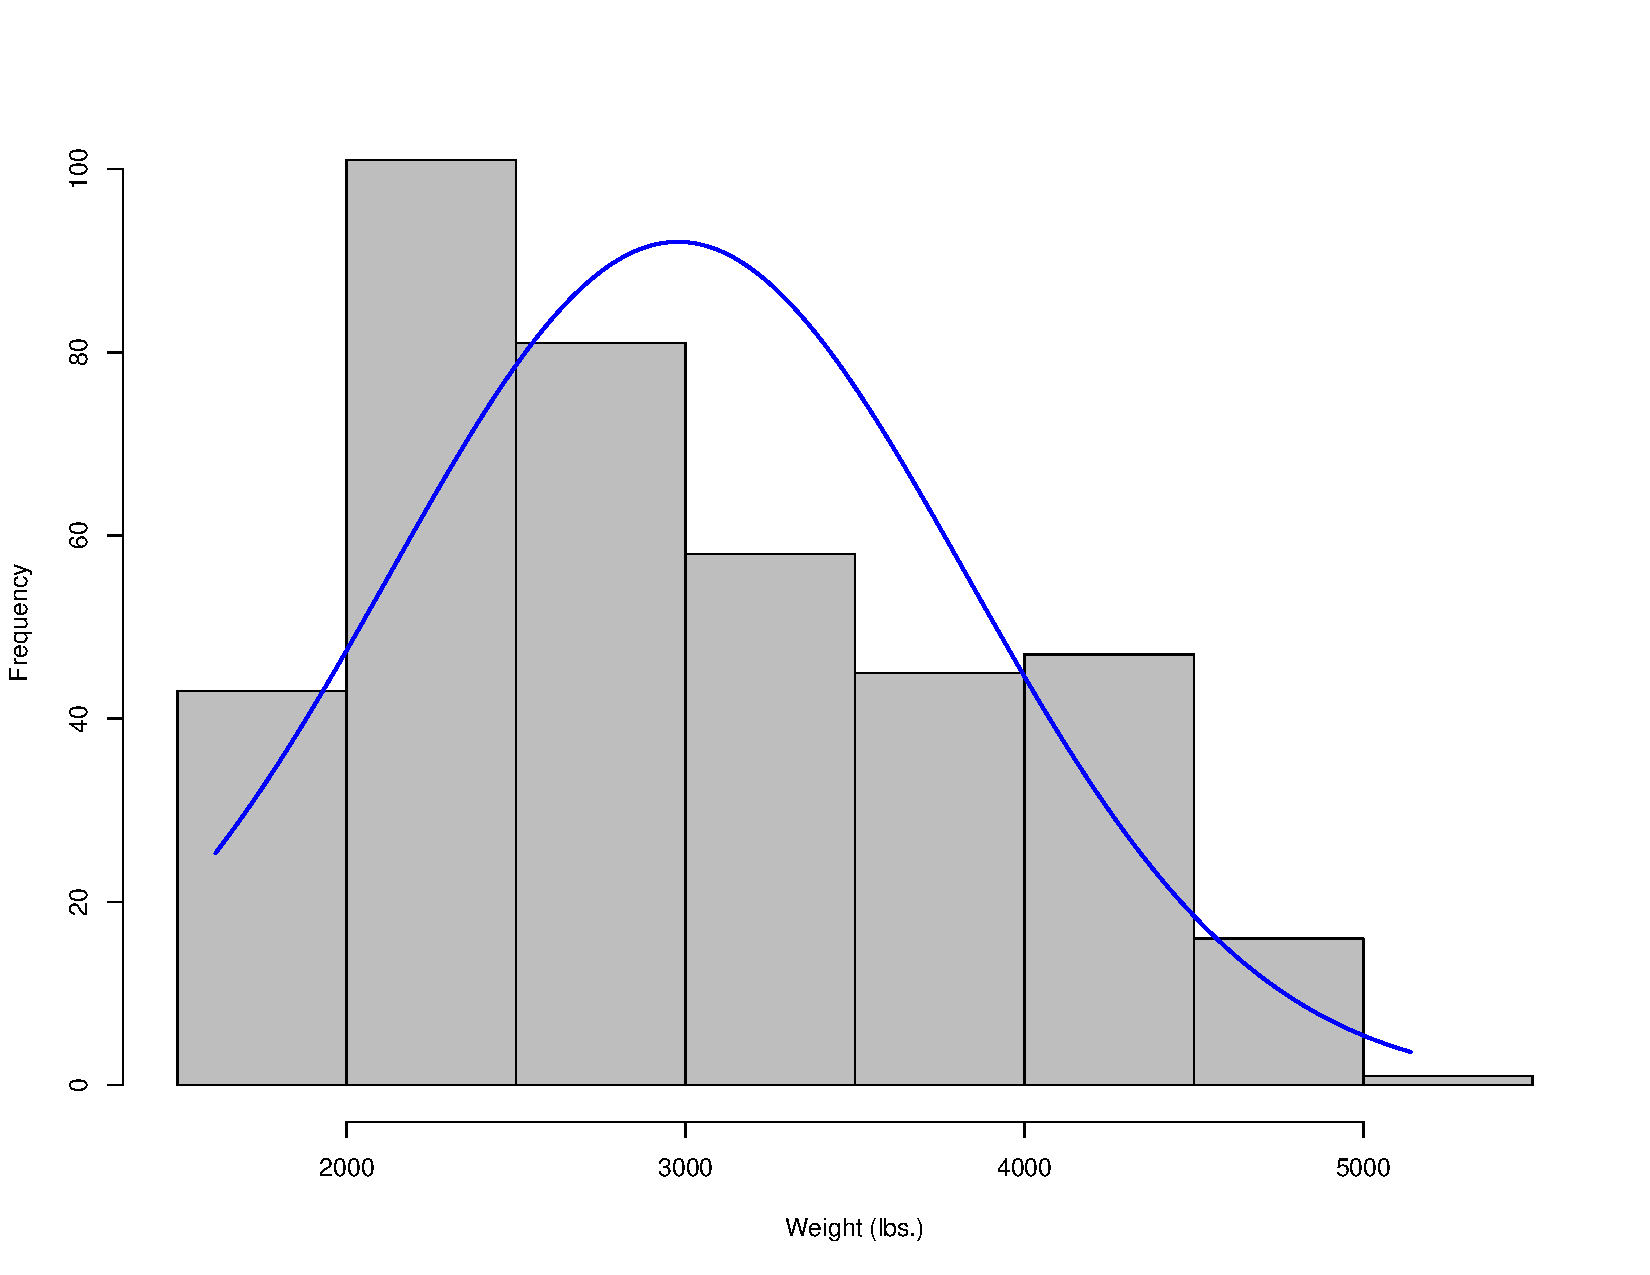
\includegraphics[width=5cm,height=4cm]{graphs/histWei.pdf}}
\subfloat[]{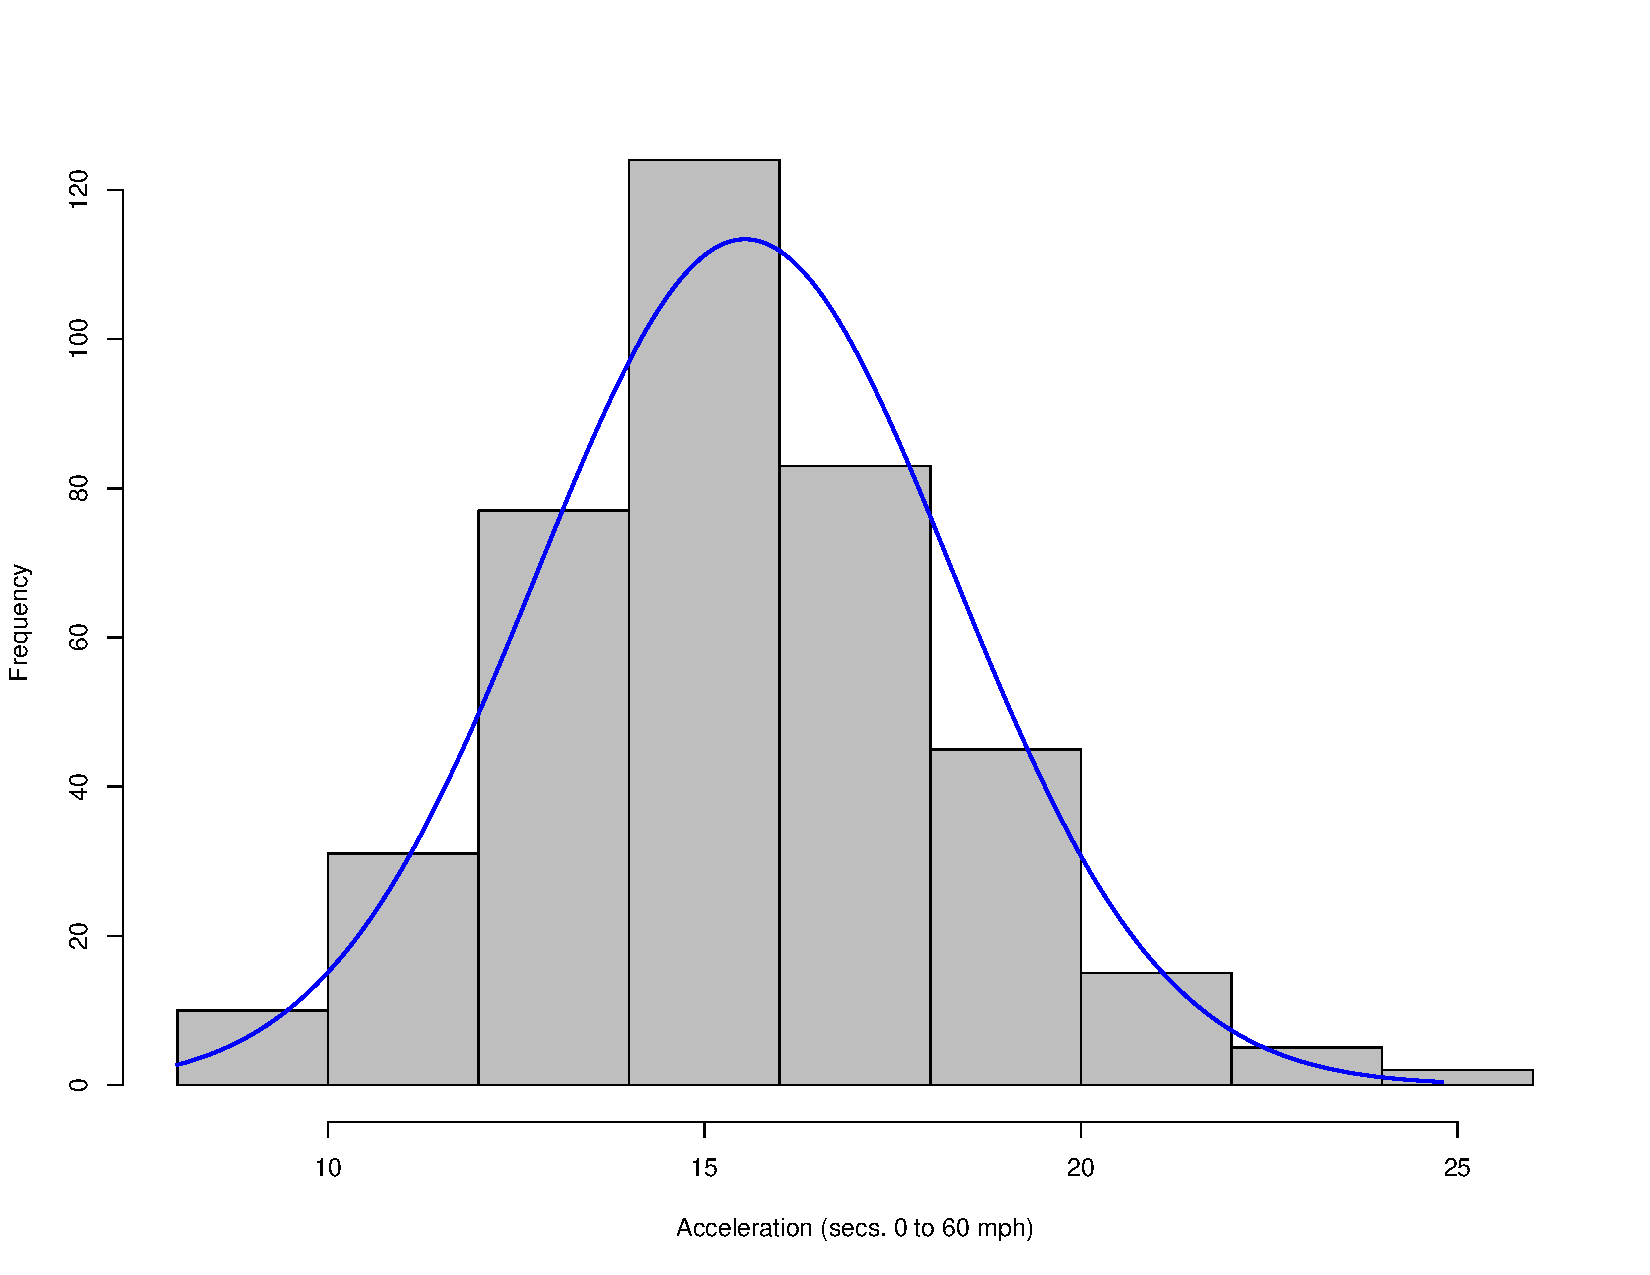
\includegraphics[width=5cm,height=4cm]{graphs/histAcc.pdf}}
\caption{Histograms of Variables}
\end{figure}

Figure 1 shows the histograms and corresponding probability density functions (pdf) of the features. Additionally, the histogram for Mpg (miles per gallon) is included. The pdfs are positioned to show the peak most clearly.
%Question 3
\question
\begin{figure}[H]
\centering
\subfloat[jittered]{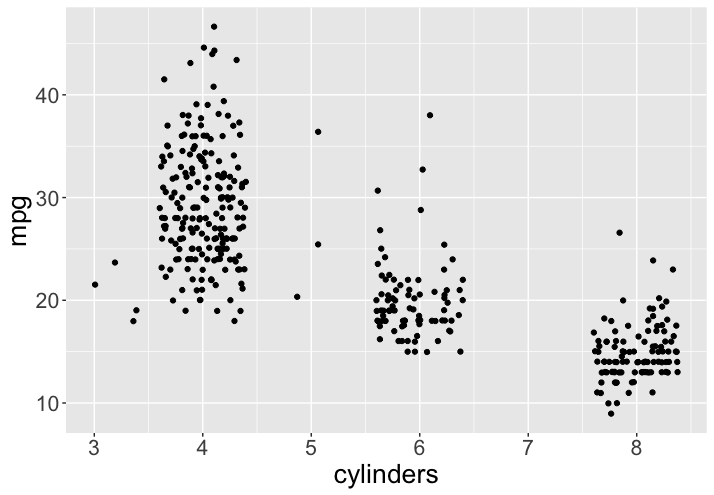
\includegraphics[width=5cm,height=4.5cm]{Images/SCT/SCTcyl.png}}
\subfloat[]{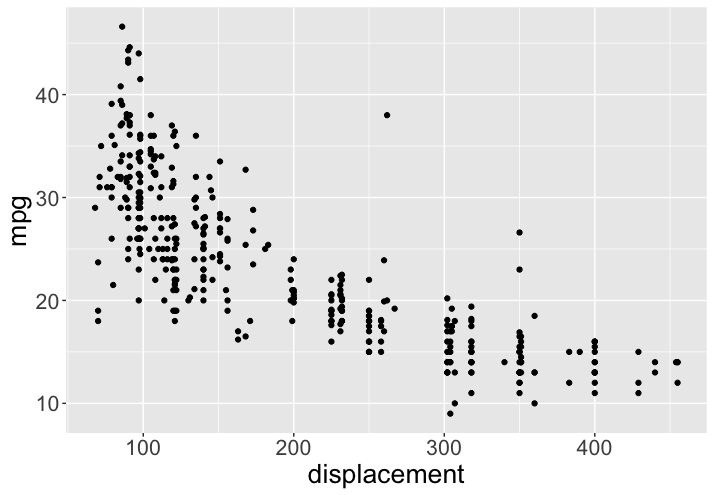
\includegraphics[width=5cm,height=4.5cm]{Images/SCT/SCTdis.png}}
\subfloat[]{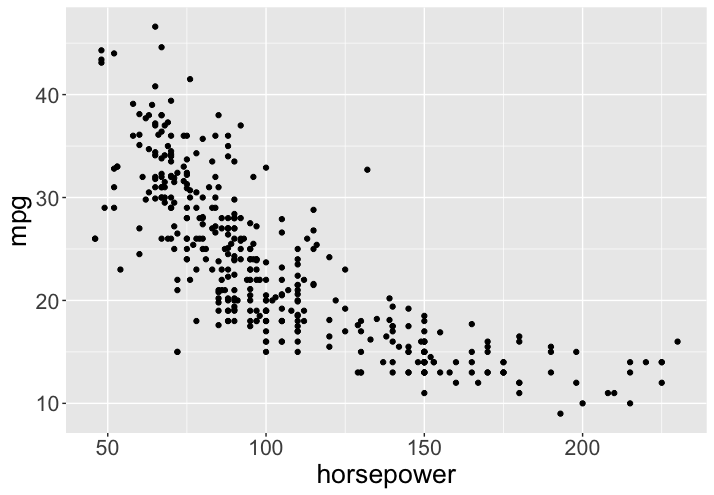
\includegraphics[width=5cm,height=4.5cm]{Images/SCT/SCThor.png}}\\
\subfloat[]{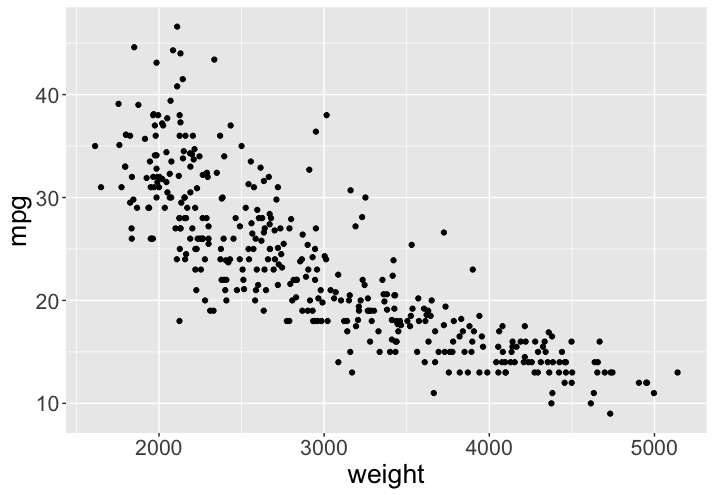
\includegraphics[width=5cm,height=4.5cm]{Images/SCT/SCTwei.png}}
\subfloat[]{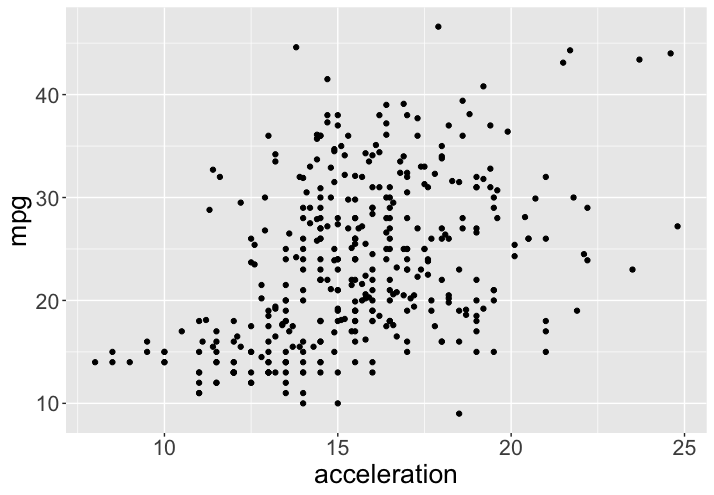
\includegraphics[width=5cm,height=4.5cm]{Images/SCT/SCTacl.png}}
\caption{Scatterplots of Features}
\end{figure}
Figure 2 shows the features as plotted against Mpg. The Cylinders feature was categorical and therefore was jittered to aid interpretation.

%Question 4
\question
The plot shows a strong negative relationship between Displacement and Mpg, which indicates that Displacement will be a good predictor for Mpg. Horsepower and Weight also appear to be good predictors for Mpg for similar reasons. The relationship between Cylinders and Mpg is less clear as Cylinders is a categorical feature. Though they appear to be negatively related, there is much variation within each class. Acceleration and Mpg appear to have no discernible relationship. From this, we expect Displacement, Horsepower and Weight to have the strongest predictive capacity for Mpg. While Cylinders may have some predictive power for mpg, Acceleration will likely have very little.
\\
\\
%Question 5
\question
\begin{rc}
           Cyl      Displ         HP     Weight     Accel
mpg -0.7776175 -0.8051269 -0.7784268 -0.8322442 0.4233285
\end{rc}
The above table of shows the correlation coefficients for both features and for Mpg. Cyl, Displ, HP, and Weight each have correlation coefficients with an absolute value greater than 0.75, indicating that they will have significant negative effects on Mpg. The value of the Acceleration correlation coefficient, 0.42, is relatively weak, so we do not expect it to impact Mpg.

%Question 6
\question
\begin{rc}
              cylinders displacement horsepower     weight acceleration
cylinders     1.0000000    0.9508233  0.8429834  0.8975273   -0.5046834
displacement  0.9508233    1.0000000  0.8972570  0.9329944   -0.5438005
horsepower    0.8429834    0.8972570  1.0000000  0.8645377   -0.6891955
weight        0.8975273    0.9329944  0.8645377  1.0000000   -0.4168392
acceleration -0.5046834   -0.5438005 -0.6891955 -0.4168392    1.0000000
\end{rc}
From the above correlation matrix, we see that most features display a strong positive correlation with each other. This can be seen through the Cylinders variable, as a greater number of Cylinders is associated with greater Displacement, higher Horsepower, and a vehicle with more Weight. The exception to this is the Acceleration feature, which instead has weak negative correlations with the other features.

%Question 7
\question
\begin{figure}[h]
    \centering
    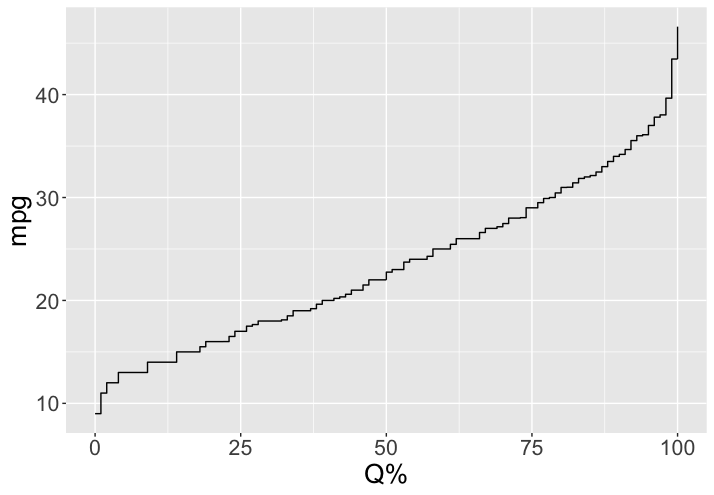
\includegraphics[width=8cm,height=6cm]{Images/Qcurve.png}
    \caption{Quantile Curve}
    \label{fig:my_label}
\end{figure}

Figure 3 shows an increasing quantile plot for the target variable, mpg. It can be interpreted by following the x-axis for a percentage of interest and checking the corresponding mpg value. For example, the 50th percentile of cars in the data set averages around 23 miles per gallon. The curve increases at a relatively consistent rate until the mid-90th percentile, when it increases steeply. This is due to some outlier vehicles that get exceptionally high gas mileage.

%Question 8
\question
The cases are split into lower and upper thirds and classed as LOWmpg and HIGHmpg, respectively. To do so we used the quantile function with a sequence of probabilities ranging from 0 to 1 in 0.01 increments and Mpg as the discriminator. Doing so splits the cases into quantiles, where the four cars with the lowest Mpg in the data set are assigned the first percent, the four with the highest Mpg are assigned the hundredth percent, and so on. The cases in LOWmpg thus spanned the 0th to 34th percentiles, and the cases in HIGHmpg spanned the 67th percentile to the 100th. This can be represented in R by the following code:
\begin{rc}
> qF = quantile(mpg,seq(0, 1, 0.01))
> LOWmpg = as.matrix(auto[mpg <= max(qF[0:34]),])
> HIGHmpg = as.matrix(auto[mpg > min(qF[67:101]),])
\end{rc}

%Question 9
\question
\begin{figure}[H]
\centering
\subfloat[]{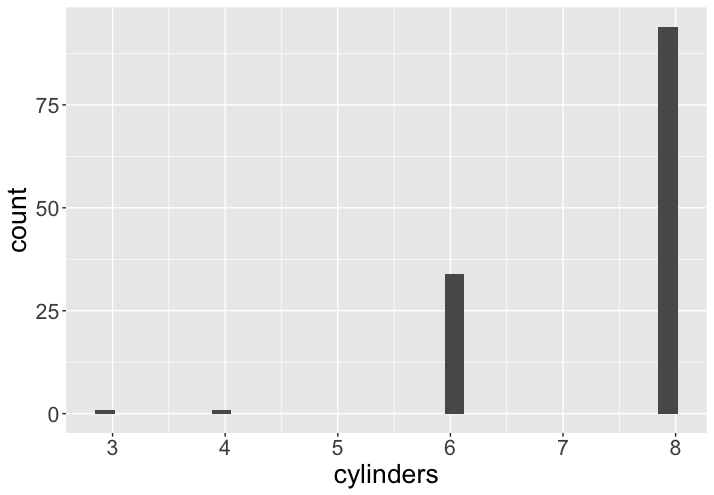
\includegraphics[width=5cm,height=4.5cm]{Images/LOW/LOWcyl.png}}
\subfloat[]{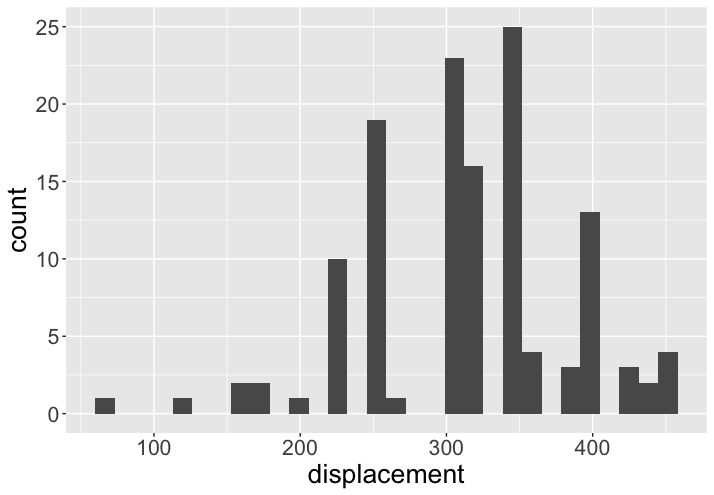
\includegraphics[width=5cm,height=4.5cm]{Images/LOW/LOWdis.png}}
\subfloat[]{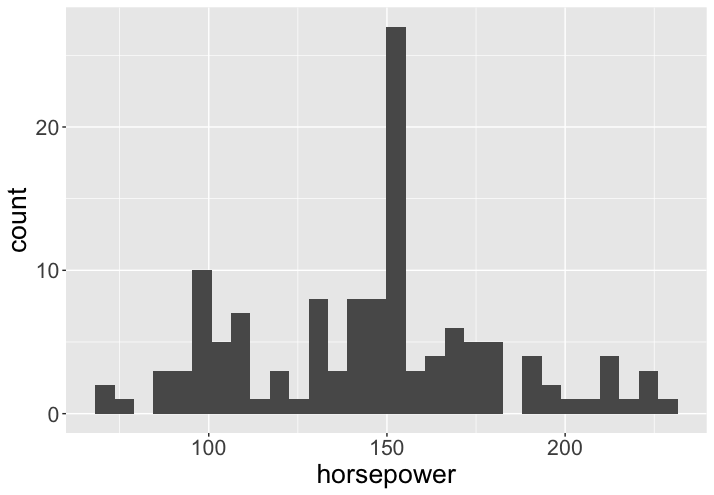
\includegraphics[width=5cm,height=4.5cm]{Images/LOW/LOWhor.png}}\\
\subfloat[]{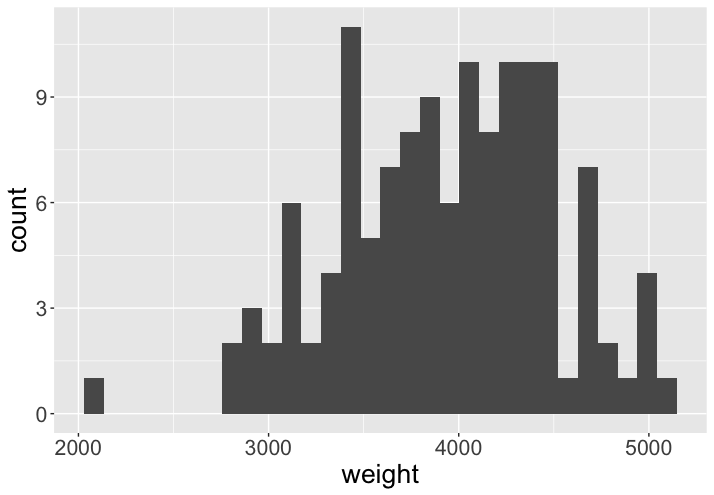
\includegraphics[width=5cm,height=4.5cm]{Images/LOW/LOWwei.png}}
\subfloat[]{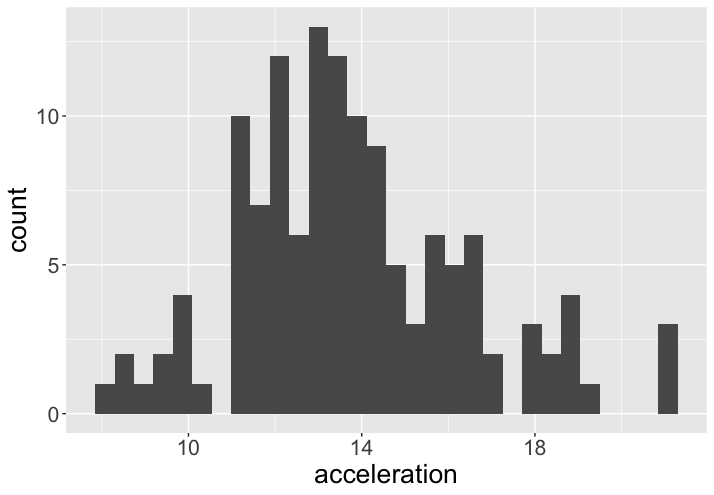
\includegraphics[width=5cm,height=4.5cm]{Images/LOW/LOWacl.png}}
\caption{Histograms for LOWmpg Features}
\end{figure}
Figure 4 shows the histograms for the features in the LOWmpg set.

\begin{figure}[H]
\centering
\subfloat[]{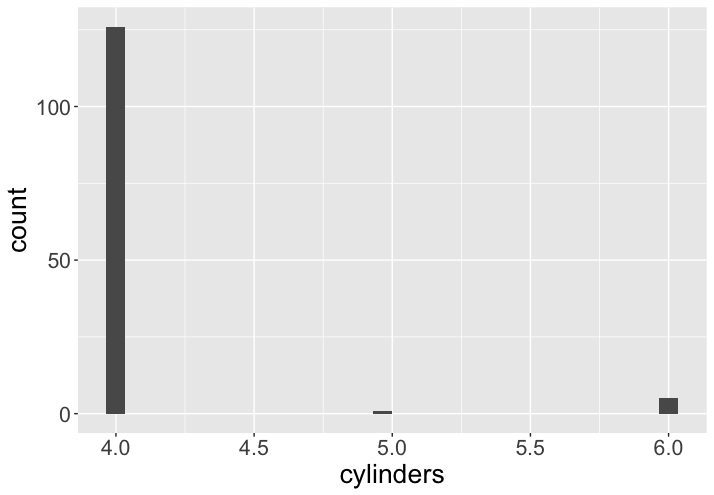
\includegraphics[width=5cm,height=4.5cm]{Images/HIGH/HIGHcyl.png}}
\subfloat[]{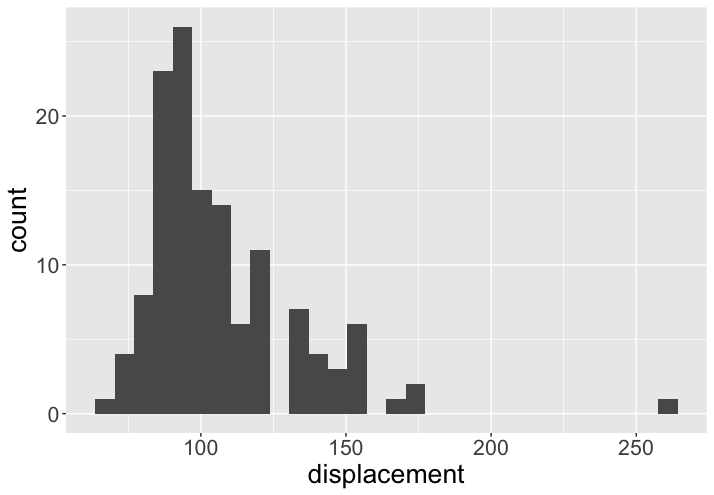
\includegraphics[width=5cm,height=4.5cm]{Images/HIGH/HIGHdis.png}}
\subfloat[]{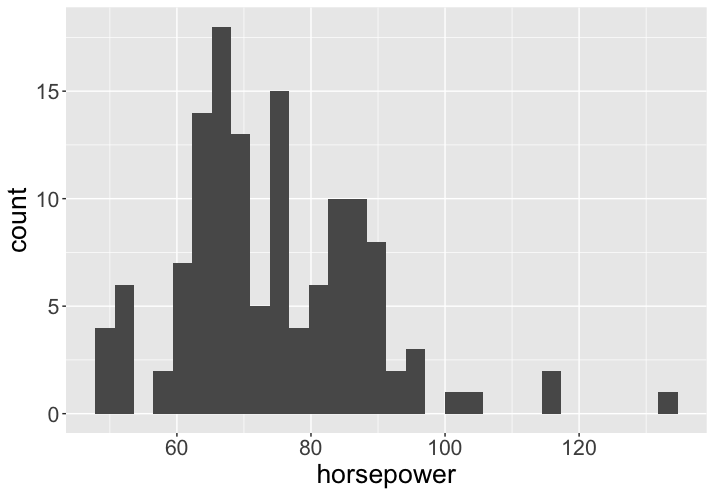
\includegraphics[width=5cm,height=4.5cm]{Images/HIGH/HIGHhor.png}}\\
\subfloat[]{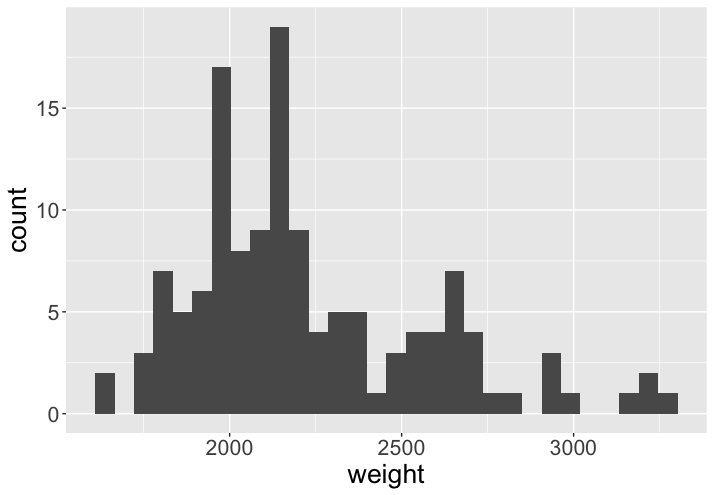
\includegraphics[width=5cm,height=4.5cm]{Images/HIGH/HIGHwei.png}}
\subfloat[]{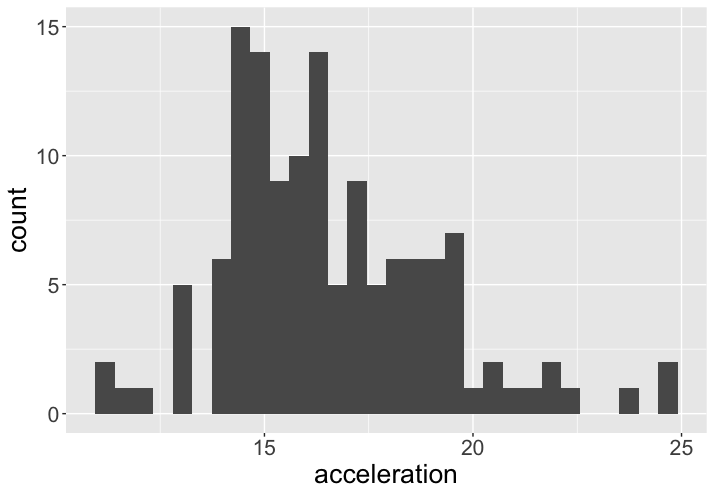
\includegraphics[width=5cm,height=4.5cm]{Images/HIGH/HIGHacl.png}}
\caption{Histograms for HIGHmpg Features}
\end{figure}

Figure 5 shows the histograms for the features in the HIGHmpg set.

%Question 10
\question
We see from the plots that the Cylinders feature shows an overwhelming majority of cars with high Mpg having four Cylinders, while most of the cars with low Mpg have six or eight Cylinders. Cars with low Displacement typically have higher Mpg, while cars with higher Displacement typically have lower Mpg, though there are outliers in both sets. The high Mpg cars typically have Horsepower values that are distributed at lower levels, while low Mpg cars have Horsepower values that are approximately normally distributed, though centered at higher levels. High Mpg cars typically weigh fewer pounds that low Mpg cars, with the former's distribution being slightly right-skew, and the latter's slightly left-skew. Acceleration is the feature closest to a normal distribution for for both high and low Mpg. 

From the plots, Cylinders appears to be a feature with strong predictive power. Additionally, a lower Displacement value could lead to higher Mpg. While it appears that cars with higher Horsepower have lower Mpg, the data is spread widely enough that further investigation of this feature is would be required.
While it appears that cars weighing over 3000 pounds have low Mpg and those weighing less than 3,000 pounds have high Mpg, this is not definite.
Concerning Acceleration, we do not see a clear difference in the values for high Mpg and low Mpg cars. As such, this feature would be the least useful in indicating if a car has low or high Mpg. In summary, Cylinders and Displacement would likely be the features with the most discriminatory power.

%Question 11
\question
LOWmpg:
\begin{rc}
            Cyl     Displ        HP    Weight     Accel
Mean   7.407692 315.30769 145.62308 3937.3308 13.778462
StdDev 1.009230  71.11404  35.84101  557.1857  2.649294
\end{rc}
HIGH mpg:
\begin{rc}
             Cyl     Displ       HP    Weight     Accel
Mean   4.0833333 106.40152 74.39394 2226.0909 16.560606
StdDev 0.3915455  26.42225 13.88434  345.8779  2.519989
\end{rc}

The above tables show the mean and standard deviation for each feature in the LOWmpg and HIGHmpg sets.
%Question 12
\question
\begin{rc}
   cylinders displacement   horsepower       weight acceleration 
   35.148517    31.517470    21.210516    29.865390     8.708918 
\end{rc}
The above table shows the discriminating ratio for each of the five features. Cylinders has the most discriminatory power, while Acceleration has the least discriminatory power. It appears Displacement and Weight also have good discriminatory power and that Horsepower may be a good indicator as well.

%Question 13
\question
For each feature, a threshold is computed as follows:
\begin{eqnarray}
thr(f)=\frac{\overline{L}\sigma_H+\overline{H}\sigma_L}{\sigma_H+\sigma_L}
\end{eqnarray}
where $\overline{L}$ and $\overline{H}$ are the mean of the feature in LOWmpg and HIGHmpg, respectively. Similarly, $\sigma_H$ and $\sigma_L$ are the standard deviation of the feature in in LOWmpg and HIGHmpg. With this, each class is given a score as follows. If $\overline{H}>\overline{L}$, the case is scored 1 if its value is above the threshold and -1 otherwise. If $\overline{L}>\overline{H}$, the case is scored 1 if it its value is below the threshold and -1 otherwise. This process is repeated for each feature of the case.
%Question 14
\question
The classes of LOWmpg and HIGHmpg are used as the training set, while the cases falling outside these are used as the test set. The true class of each case is considered low if its Mpg is below the median Mpg value and high if it is above. Consequently, all cases in the LOWmpg set will have class low and all cases in HIGHmpg will have class high, as these sets lie firmly on those respective sided of the median. For the prediction, an automatic classifier is used. The classifier uses the sum of the feature scores (known as the full score) for each case and a chosen value A. Case are classed as low Mpg if their score was less than A and as high Mpg otherwise. 
\\
Starting with an A value of 1, applying the classifier to the training and test set gives the following results:
\begin{table}[H]
    \centering
    \subfloat[train]{\begin{tabular}{c|c c}
    &low&high\\ \hline
    low&0.99230769&0.007692308\\
    high&0.03030303&0.969696970
    \end{tabular}}
    \subfloat[test]{\begin{tabular}{c|c c}
    &low&high\\ \hline
    low&0.6666667&0.3333333\\
    high&0.1406250&0.8593750
    \end{tabular}}
    \caption{Confusion Matrix. True class is by row, Predicted class is by column}
    \label{tab:my_label}
\end{table}

From the confusion matrix we see that when A=1 the classifier has high accuracy for the training set. Of the 130 total lowMPG cases, it was able to properly identify 129, and it only incorrectly labeled 4 of the 132 highMPG cases. When applied to the test set, there is a noticeable drop in accuracy. It was able to correctly label 55 of the 64 high Mpg cases and only 44 of the 66 low Mpg cases. In total, the global accuracy is 98.01\% for the training set and 76.15\% for the test set.

Moving onto an A value of 2, we get:
\begin{table}[H]
    \centering
    \subfloat[train]{\begin{tabular}{c|c c}
    &low&high\\ \hline
    low&0.99230769&0.007692308\\
    high&0.07575758&0.924242424
    \end{tabular}}
    \subfloat[test]{\begin{tabular}{c|c c}
    &low&high\\ \hline
    low&0.7575758&0.2424242\\
    high&0.3281250&0.6718750
    \end{tabular}}
    \caption{Confusion Matrix. True class is by row, Predicted class is by column}
    \label{tab:my_label}
\end{table}
The classifier's accuracy decreased for the training set and gave mixed results for the test set. For the training set, the low Mpg numbers are the same as they were previously. However, the classifier did a worse job identifying high Mpg cases with a 4.5\% decrease in accuracy. For the test set the classifier does a better job identifying the low Mpg cases but a worse job for the high Mpg cases. It shows approximately a 9.1\% increase in accuracy for low mpg cases and a 18.75\%  decrease in accuracy high mpg cases. The global accuracy for the training set is 95.8\%, while for the test set it is 71.54\%

Since the list of full scores for both sets only contain odd values (ranging from -5 to 5), any even value A will have the same results as A=A+1. Therefore, the results for A=0 is the same as for A=1 and A=3 is the same as A=2. From the confusion matrices and global accuracy values corresponding to each set, we conclude that a value of 1 for A is most effective as it gives the least amount of disparity in classification.

The differences between the results for the training set and the test set may suggest that there is over fitting of the training data. The threshold levels for the classifier function, which were determined from the standard deviations found in the training set, appear to serve very well in classifying the training set at any value of A but are much less adequate for the test set. Optimizing the A value is not enough to improve this automatic classifier. We may need to revise the calculation for thr(F) to be more effective. 

\newpage
\lstinputlisting{code.R}
\end{document}
